% Created by tikzDevice version 0.6.2-92-0ad2792 on 2013-03-28 13:08:00
% !TEX encoding = UTF-8 Unicode
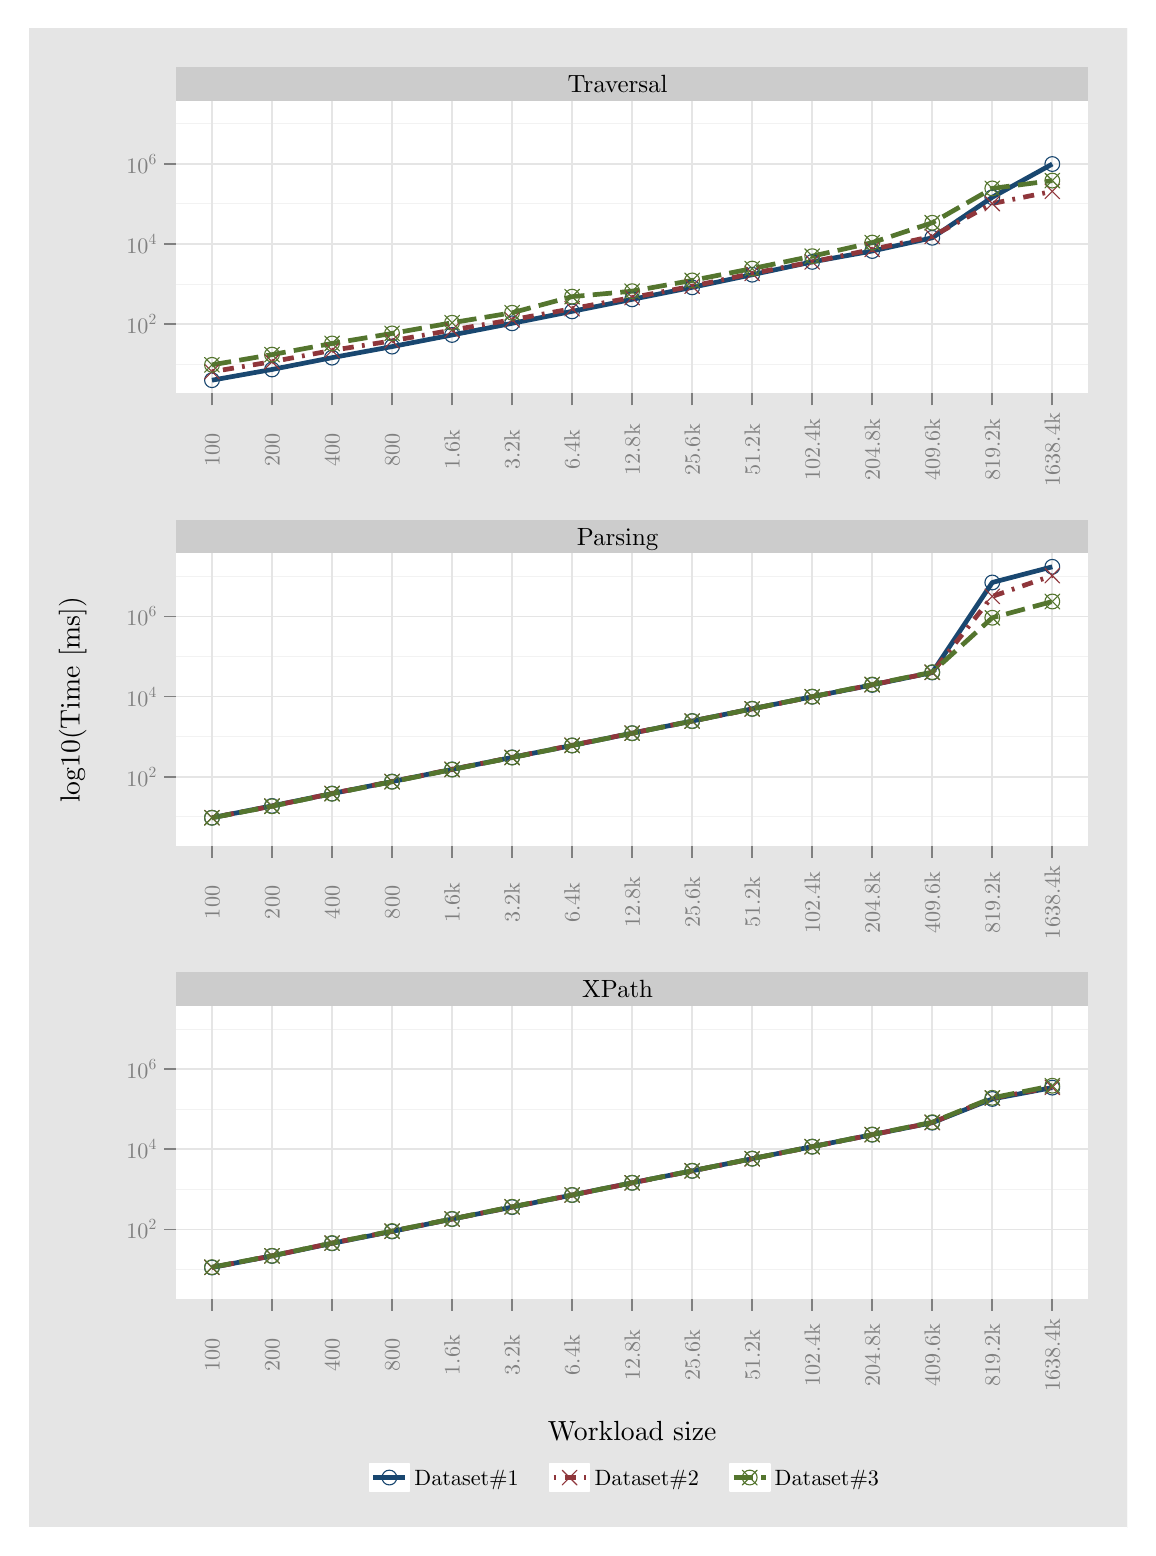
\begin{tikzpicture}[x=1pt,y=1pt]
\definecolor[named]{fillColor}{rgb}{1.00,1.00,1.00}
\path[use as bounding box,fill=fillColor,fill opacity=0.00] (0,0) rectangle (397.48,542.02);
\begin{scope}
\path[clip] (  0.00,  0.00) rectangle (397.48,542.02);
\definecolor[named]{drawColor}{rgb}{1.00,1.00,1.00}
\definecolor[named]{fillColor}{rgb}{0.90,0.90,0.90}

\path[draw=drawColor,line width= 0.6pt,line join=round,line cap=round,fill=fillColor] (  0.00,  0.00) rectangle (397.48,542.02);
\end{scope}
\begin{scope}
\path[clip] ( 53.58,409.83) rectangle (383.26,515.58);
\definecolor[named]{fillColor}{rgb}{1.00,1.00,1.00}

\path[fill=fillColor] ( 53.58,409.83) rectangle (383.26,515.58);
\definecolor[named]{drawColor}{rgb}{0.95,0.95,0.95}

\path[draw=drawColor,line width= 0.3pt,line join=round] ( 53.58,420.43) --
	(383.26,420.43);

\path[draw=drawColor,line width= 0.3pt,line join=round] ( 53.58,449.39) --
	(383.26,449.39);

\path[draw=drawColor,line width= 0.3pt,line join=round] ( 53.58,478.35) --
	(383.26,478.35);

\path[draw=drawColor,line width= 0.3pt,line join=round] ( 53.58,507.31) --
	(383.26,507.31);
\definecolor[named]{drawColor}{rgb}{0.90,0.90,0.90}

\path[draw=drawColor,line width= 0.6pt,line join=round] ( 53.58,434.91) --
	(383.26,434.91);

\path[draw=drawColor,line width= 0.6pt,line join=round] ( 53.58,463.87) --
	(383.26,463.87);

\path[draw=drawColor,line width= 0.6pt,line join=round] ( 53.58,492.83) --
	(383.26,492.83);

\path[draw=drawColor,line width= 0.6pt,line join=round] ( 66.60,409.83) --
	( 66.60,515.58);

\path[draw=drawColor,line width= 0.6pt,line join=round] ( 88.29,409.83) --
	( 88.29,515.58);

\path[draw=drawColor,line width= 0.6pt,line join=round] (109.97,409.83) --
	(109.97,515.58);

\path[draw=drawColor,line width= 0.6pt,line join=round] (131.66,409.83) --
	(131.66,515.58);

\path[draw=drawColor,line width= 0.6pt,line join=round] (153.35,409.83) --
	(153.35,515.58);

\path[draw=drawColor,line width= 0.6pt,line join=round] (175.04,409.83) --
	(175.04,515.58);

\path[draw=drawColor,line width= 0.6pt,line join=round] (196.73,409.83) --
	(196.73,515.58);

\path[draw=drawColor,line width= 0.6pt,line join=round] (218.42,409.83) --
	(218.42,515.58);

\path[draw=drawColor,line width= 0.6pt,line join=round] (240.11,409.83) --
	(240.11,515.58);

\path[draw=drawColor,line width= 0.6pt,line join=round] (261.80,409.83) --
	(261.80,515.58);

\path[draw=drawColor,line width= 0.6pt,line join=round] (283.49,409.83) --
	(283.49,515.58);

\path[draw=drawColor,line width= 0.6pt,line join=round] (305.18,409.83) --
	(305.18,515.58);

\path[draw=drawColor,line width= 0.6pt,line join=round] (326.87,409.83) --
	(326.87,515.58);

\path[draw=drawColor,line width= 0.6pt,line join=round] (348.56,409.83) --
	(348.56,515.58);

\path[draw=drawColor,line width= 0.6pt,line join=round] (370.25,409.83) --
	(370.25,515.58);
\definecolor[named]{drawColor}{rgb}{0.10,0.28,0.44}

\path[draw=drawColor,line width= 1.7pt,line join=round] ( 66.60,414.63) --
	( 88.29,418.51) --
	(109.97,422.77) --
	(131.66,426.77) --
	(153.35,430.97) --
	(175.04,435.18) --
	(196.73,439.50) --
	(218.42,443.85) --
	(240.11,448.18) --
	(261.80,452.75) --
	(283.49,457.38) --
	(305.18,461.31) --
	(326.87,466.09) --
	(348.56,480.74) --
	(370.25,492.74);
\definecolor[named]{drawColor}{rgb}{0.56,0.21,0.23}

\path[draw=drawColor,line width= 1.7pt,dash pattern=on 1pt off 3pt on 4pt off 3pt ,line join=round] ( 66.60,417.70) --
	( 88.29,421.31) --
	(109.97,425.39) --
	(131.66,428.85) --
	(153.35,432.75) --
	(175.04,436.47) --
	(196.73,440.47) --
	(218.42,444.51) --
	(240.11,448.60) --
	(261.80,453.20) --
	(283.49,457.39) --
	(305.18,461.88) --
	(326.87,466.61) --
	(348.56,478.47) --
	(370.25,482.86);
\definecolor[named]{drawColor}{rgb}{0.33,0.46,0.18}

\path[draw=drawColor,line width= 1.7pt,dash pattern=on 7pt off 3pt ,line join=round] ( 66.60,420.18) --
	( 88.29,423.87) --
	(109.97,427.90) --
	(131.66,431.53) --
	(153.35,435.39) --
	(175.04,439.00) --
	(196.73,444.82) --
	(218.42,446.79) --
	(240.11,450.68) --
	(261.80,454.96) --
	(283.49,459.44) --
	(305.18,464.35) --
	(326.87,471.52) --
	(348.56,483.93) --
	(370.25,486.76);
\definecolor[named]{drawColor}{rgb}{0.10,0.28,0.44}

\path[draw=drawColor,line width= 0.4pt,line join=round,line cap=round] ( 66.60,414.63) circle (  2.67);

\path[draw=drawColor,line width= 0.4pt,line join=round,line cap=round] ( 88.29,418.51) circle (  2.67);

\path[draw=drawColor,line width= 0.4pt,line join=round,line cap=round] (109.97,422.77) circle (  2.67);

\path[draw=drawColor,line width= 0.4pt,line join=round,line cap=round] (131.66,426.77) circle (  2.67);

\path[draw=drawColor,line width= 0.4pt,line join=round,line cap=round] (153.35,430.97) circle (  2.67);

\path[draw=drawColor,line width= 0.4pt,line join=round,line cap=round] (175.04,435.18) circle (  2.67);

\path[draw=drawColor,line width= 0.4pt,line join=round,line cap=round] (196.73,439.50) circle (  2.67);

\path[draw=drawColor,line width= 0.4pt,line join=round,line cap=round] (218.42,443.85) circle (  2.67);

\path[draw=drawColor,line width= 0.4pt,line join=round,line cap=round] (240.11,448.18) circle (  2.67);

\path[draw=drawColor,line width= 0.4pt,line join=round,line cap=round] (261.80,452.75) circle (  2.67);

\path[draw=drawColor,line width= 0.4pt,line join=round,line cap=round] (283.49,457.38) circle (  2.67);

\path[draw=drawColor,line width= 0.4pt,line join=round,line cap=round] (305.18,461.31) circle (  2.67);

\path[draw=drawColor,line width= 0.4pt,line join=round,line cap=round] (326.87,466.09) circle (  2.67);

\path[draw=drawColor,line width= 0.4pt,line join=round,line cap=round] (348.56,480.74) circle (  2.67);

\path[draw=drawColor,line width= 0.4pt,line join=round,line cap=round] (370.25,492.74) circle (  2.67);
\definecolor[named]{drawColor}{rgb}{0.56,0.21,0.23}

\path[draw=drawColor,line width= 0.4pt,line join=round,line cap=round] ( 63.93,415.04) -- ( 69.26,420.37);

\path[draw=drawColor,line width= 0.4pt,line join=round,line cap=round] ( 63.93,420.37) -- ( 69.26,415.04);

\path[draw=drawColor,line width= 0.4pt,line join=round,line cap=round] ( 85.62,418.64) -- ( 90.95,423.97);

\path[draw=drawColor,line width= 0.4pt,line join=round,line cap=round] ( 85.62,423.97) -- ( 90.95,418.64);

\path[draw=drawColor,line width= 0.4pt,line join=round,line cap=round] (107.31,422.72) -- (112.64,428.06);

\path[draw=drawColor,line width= 0.4pt,line join=round,line cap=round] (107.31,428.06) -- (112.64,422.72);

\path[draw=drawColor,line width= 0.4pt,line join=round,line cap=round] (129.00,426.18) -- (134.33,431.52);

\path[draw=drawColor,line width= 0.4pt,line join=round,line cap=round] (129.00,431.52) -- (134.33,426.18);

\path[draw=drawColor,line width= 0.4pt,line join=round,line cap=round] (150.69,430.08) -- (156.02,435.42);

\path[draw=drawColor,line width= 0.4pt,line join=round,line cap=round] (150.69,435.42) -- (156.02,430.08);

\path[draw=drawColor,line width= 0.4pt,line join=round,line cap=round] (172.37,433.80) -- (177.71,439.14);

\path[draw=drawColor,line width= 0.4pt,line join=round,line cap=round] (172.37,439.14) -- (177.71,433.80);

\path[draw=drawColor,line width= 0.4pt,line join=round,line cap=round] (194.06,437.80) -- (199.40,443.14);

\path[draw=drawColor,line width= 0.4pt,line join=round,line cap=round] (194.06,443.14) -- (199.40,437.80);

\path[draw=drawColor,line width= 0.4pt,line join=round,line cap=round] (215.75,441.84) -- (221.09,447.18);

\path[draw=drawColor,line width= 0.4pt,line join=round,line cap=round] (215.75,447.18) -- (221.09,441.84);

\path[draw=drawColor,line width= 0.4pt,line join=round,line cap=round] (237.44,445.93) -- (242.78,451.26);

\path[draw=drawColor,line width= 0.4pt,line join=round,line cap=round] (237.44,451.26) -- (242.78,445.93);

\path[draw=drawColor,line width= 0.4pt,line join=round,line cap=round] (259.13,450.53) -- (264.47,455.87);

\path[draw=drawColor,line width= 0.4pt,line join=round,line cap=round] (259.13,455.87) -- (264.47,450.53);

\path[draw=drawColor,line width= 0.4pt,line join=round,line cap=round] (280.82,454.73) -- (286.16,460.06);

\path[draw=drawColor,line width= 0.4pt,line join=round,line cap=round] (280.82,460.06) -- (286.16,454.73);

\path[draw=drawColor,line width= 0.4pt,line join=round,line cap=round] (302.51,459.21) -- (307.84,464.54);

\path[draw=drawColor,line width= 0.4pt,line join=round,line cap=round] (302.51,464.54) -- (307.84,459.21);

\path[draw=drawColor,line width= 0.4pt,line join=round,line cap=round] (324.20,463.94) -- (329.53,469.28);

\path[draw=drawColor,line width= 0.4pt,line join=round,line cap=round] (324.20,469.28) -- (329.53,463.94);

\path[draw=drawColor,line width= 0.4pt,line join=round,line cap=round] (345.89,475.80) -- (351.22,481.13);

\path[draw=drawColor,line width= 0.4pt,line join=round,line cap=round] (345.89,481.13) -- (351.22,475.80);

\path[draw=drawColor,line width= 0.4pt,line join=round,line cap=round] (367.58,480.19) -- (372.91,485.52);

\path[draw=drawColor,line width= 0.4pt,line join=round,line cap=round] (367.58,485.52) -- (372.91,480.19);
\definecolor[named]{drawColor}{rgb}{0.33,0.46,0.18}

\path[draw=drawColor,line width= 0.4pt,line join=round,line cap=round] ( 66.60,420.18) circle (  2.67);

\path[draw=drawColor,line width= 0.4pt,line join=round,line cap=round] ( 63.93,417.51) -- ( 69.26,422.85);

\path[draw=drawColor,line width= 0.4pt,line join=round,line cap=round] ( 63.93,422.85) -- ( 69.26,417.51);

\path[draw=drawColor,line width= 0.4pt,line join=round,line cap=round] ( 88.29,423.87) circle (  2.67);

\path[draw=drawColor,line width= 0.4pt,line join=round,line cap=round] ( 85.62,421.20) -- ( 90.95,426.53);

\path[draw=drawColor,line width= 0.4pt,line join=round,line cap=round] ( 85.62,426.53) -- ( 90.95,421.20);

\path[draw=drawColor,line width= 0.4pt,line join=round,line cap=round] (109.97,427.90) circle (  2.67);

\path[draw=drawColor,line width= 0.4pt,line join=round,line cap=round] (107.31,425.23) -- (112.64,430.57);

\path[draw=drawColor,line width= 0.4pt,line join=round,line cap=round] (107.31,430.57) -- (112.64,425.23);

\path[draw=drawColor,line width= 0.4pt,line join=round,line cap=round] (131.66,431.53) circle (  2.67);

\path[draw=drawColor,line width= 0.4pt,line join=round,line cap=round] (129.00,428.86) -- (134.33,434.20);

\path[draw=drawColor,line width= 0.4pt,line join=round,line cap=round] (129.00,434.20) -- (134.33,428.86);

\path[draw=drawColor,line width= 0.4pt,line join=round,line cap=round] (153.35,435.39) circle (  2.67);

\path[draw=drawColor,line width= 0.4pt,line join=round,line cap=round] (150.69,432.72) -- (156.02,438.06);

\path[draw=drawColor,line width= 0.4pt,line join=round,line cap=round] (150.69,438.06) -- (156.02,432.72);

\path[draw=drawColor,line width= 0.4pt,line join=round,line cap=round] (175.04,439.00) circle (  2.67);

\path[draw=drawColor,line width= 0.4pt,line join=round,line cap=round] (172.37,436.34) -- (177.71,441.67);

\path[draw=drawColor,line width= 0.4pt,line join=round,line cap=round] (172.37,441.67) -- (177.71,436.34);

\path[draw=drawColor,line width= 0.4pt,line join=round,line cap=round] (196.73,444.82) circle (  2.67);

\path[draw=drawColor,line width= 0.4pt,line join=round,line cap=round] (194.06,442.16) -- (199.40,447.49);

\path[draw=drawColor,line width= 0.4pt,line join=round,line cap=round] (194.06,447.49) -- (199.40,442.16);

\path[draw=drawColor,line width= 0.4pt,line join=round,line cap=round] (218.42,446.79) circle (  2.67);

\path[draw=drawColor,line width= 0.4pt,line join=round,line cap=round] (215.75,444.12) -- (221.09,449.46);

\path[draw=drawColor,line width= 0.4pt,line join=round,line cap=round] (215.75,449.46) -- (221.09,444.12);

\path[draw=drawColor,line width= 0.4pt,line join=round,line cap=round] (240.11,450.68) circle (  2.67);

\path[draw=drawColor,line width= 0.4pt,line join=round,line cap=round] (237.44,448.02) -- (242.78,453.35);

\path[draw=drawColor,line width= 0.4pt,line join=round,line cap=round] (237.44,453.35) -- (242.78,448.02);

\path[draw=drawColor,line width= 0.4pt,line join=round,line cap=round] (261.80,454.96) circle (  2.67);

\path[draw=drawColor,line width= 0.4pt,line join=round,line cap=round] (259.13,452.29) -- (264.47,457.62);

\path[draw=drawColor,line width= 0.4pt,line join=round,line cap=round] (259.13,457.62) -- (264.47,452.29);

\path[draw=drawColor,line width= 0.4pt,line join=round,line cap=round] (283.49,459.44) circle (  2.67);

\path[draw=drawColor,line width= 0.4pt,line join=round,line cap=round] (280.82,456.78) -- (286.16,462.11);

\path[draw=drawColor,line width= 0.4pt,line join=round,line cap=round] (280.82,462.11) -- (286.16,456.78);

\path[draw=drawColor,line width= 0.4pt,line join=round,line cap=round] (305.18,464.35) circle (  2.67);

\path[draw=drawColor,line width= 0.4pt,line join=round,line cap=round] (302.51,461.68) -- (307.84,467.02);

\path[draw=drawColor,line width= 0.4pt,line join=round,line cap=round] (302.51,467.02) -- (307.84,461.68);

\path[draw=drawColor,line width= 0.4pt,line join=round,line cap=round] (326.87,471.52) circle (  2.67);

\path[draw=drawColor,line width= 0.4pt,line join=round,line cap=round] (324.20,468.86) -- (329.53,474.19);

\path[draw=drawColor,line width= 0.4pt,line join=round,line cap=round] (324.20,474.19) -- (329.53,468.86);

\path[draw=drawColor,line width= 0.4pt,line join=round,line cap=round] (348.56,483.93) circle (  2.67);

\path[draw=drawColor,line width= 0.4pt,line join=round,line cap=round] (345.89,481.27) -- (351.22,486.60);

\path[draw=drawColor,line width= 0.4pt,line join=round,line cap=round] (345.89,486.60) -- (351.22,481.27);

\path[draw=drawColor,line width= 0.4pt,line join=round,line cap=round] (370.25,486.76) circle (  2.67);

\path[draw=drawColor,line width= 0.4pt,line join=round,line cap=round] (367.58,484.10) -- (372.91,489.43);

\path[draw=drawColor,line width= 0.4pt,line join=round,line cap=round] (367.58,489.43) -- (372.91,484.10);
\end{scope}
\begin{scope}
\path[clip] ( 53.58,246.26) rectangle (383.26,352.01);
\definecolor[named]{fillColor}{rgb}{1.00,1.00,1.00}

\path[fill=fillColor] ( 53.58,246.26) rectangle (383.26,352.01);
\definecolor[named]{drawColor}{rgb}{0.95,0.95,0.95}

\path[draw=drawColor,line width= 0.3pt,line join=round] ( 53.58,256.86) --
	(383.26,256.86);

\path[draw=drawColor,line width= 0.3pt,line join=round] ( 53.58,285.82) --
	(383.26,285.82);

\path[draw=drawColor,line width= 0.3pt,line join=round] ( 53.58,314.78) --
	(383.26,314.78);

\path[draw=drawColor,line width= 0.3pt,line join=round] ( 53.58,343.74) --
	(383.26,343.74);
\definecolor[named]{drawColor}{rgb}{0.90,0.90,0.90}

\path[draw=drawColor,line width= 0.6pt,line join=round] ( 53.58,271.34) --
	(383.26,271.34);

\path[draw=drawColor,line width= 0.6pt,line join=round] ( 53.58,300.30) --
	(383.26,300.30);

\path[draw=drawColor,line width= 0.6pt,line join=round] ( 53.58,329.26) --
	(383.26,329.26);

\path[draw=drawColor,line width= 0.6pt,line join=round] ( 66.60,246.26) --
	( 66.60,352.01);

\path[draw=drawColor,line width= 0.6pt,line join=round] ( 88.29,246.26) --
	( 88.29,352.01);

\path[draw=drawColor,line width= 0.6pt,line join=round] (109.97,246.26) --
	(109.97,352.01);

\path[draw=drawColor,line width= 0.6pt,line join=round] (131.66,246.26) --
	(131.66,352.01);

\path[draw=drawColor,line width= 0.6pt,line join=round] (153.35,246.26) --
	(153.35,352.01);

\path[draw=drawColor,line width= 0.6pt,line join=round] (175.04,246.26) --
	(175.04,352.01);

\path[draw=drawColor,line width= 0.6pt,line join=round] (196.73,246.26) --
	(196.73,352.01);

\path[draw=drawColor,line width= 0.6pt,line join=round] (218.42,246.26) --
	(218.42,352.01);

\path[draw=drawColor,line width= 0.6pt,line join=round] (240.11,246.26) --
	(240.11,352.01);

\path[draw=drawColor,line width= 0.6pt,line join=round] (261.80,246.26) --
	(261.80,352.01);

\path[draw=drawColor,line width= 0.6pt,line join=round] (283.49,246.26) --
	(283.49,352.01);

\path[draw=drawColor,line width= 0.6pt,line join=round] (305.18,246.26) --
	(305.18,352.01);

\path[draw=drawColor,line width= 0.6pt,line join=round] (326.87,246.26) --
	(326.87,352.01);

\path[draw=drawColor,line width= 0.6pt,line join=round] (348.56,246.26) --
	(348.56,352.01);

\path[draw=drawColor,line width= 0.6pt,line join=round] (370.25,246.26) --
	(370.25,352.01);
\definecolor[named]{drawColor}{rgb}{0.10,0.28,0.44}

\path[draw=drawColor,line width= 1.7pt,line join=round] ( 66.60,256.53) --
	( 88.29,260.80) --
	(109.97,265.25) --
	(131.66,269.59) --
	(153.35,273.99) --
	(175.04,278.33) --
	(196.73,282.64) --
	(218.42,287.08) --
	(240.11,291.47) --
	(261.80,295.89) --
	(283.49,300.25) --
	(305.18,304.52) --
	(326.87,309.01) --
	(348.56,341.54) --
	(370.25,347.20);
\definecolor[named]{drawColor}{rgb}{0.56,0.21,0.23}

\path[draw=drawColor,line width= 1.7pt,dash pattern=on 1pt off 3pt on 4pt off 3pt ,line join=round] ( 66.60,256.55) --
	( 88.29,260.73) --
	(109.97,265.29) --
	(131.66,269.61) --
	(153.35,274.04) --
	(175.04,278.34) --
	(196.73,282.74) --
	(218.42,287.11) --
	(240.11,291.47) --
	(261.80,295.84) --
	(283.49,300.22) --
	(305.18,304.58) --
	(326.87,309.01) --
	(348.56,336.51) --
	(370.25,344.03);
\definecolor[named]{drawColor}{rgb}{0.33,0.46,0.18}

\path[draw=drawColor,line width= 1.7pt,dash pattern=on 7pt off 3pt ,line join=round] ( 66.60,256.51) --
	( 88.29,260.67) --
	(109.97,265.20) --
	(131.66,269.52) --
	(153.35,273.92) --
	(175.04,278.27) --
	(196.73,282.64) --
	(218.42,287.06) --
	(240.11,291.43) --
	(261.80,295.87) --
	(283.49,300.28) --
	(305.18,304.67) --
	(326.87,309.13) --
	(348.56,328.79) --
	(370.25,334.66);
\definecolor[named]{drawColor}{rgb}{0.10,0.28,0.44}

\path[draw=drawColor,line width= 0.4pt,line join=round,line cap=round] ( 66.60,256.53) circle (  2.67);

\path[draw=drawColor,line width= 0.4pt,line join=round,line cap=round] ( 88.29,260.80) circle (  2.67);

\path[draw=drawColor,line width= 0.4pt,line join=round,line cap=round] (109.97,265.25) circle (  2.67);

\path[draw=drawColor,line width= 0.4pt,line join=round,line cap=round] (131.66,269.59) circle (  2.67);

\path[draw=drawColor,line width= 0.4pt,line join=round,line cap=round] (153.35,273.99) circle (  2.67);

\path[draw=drawColor,line width= 0.4pt,line join=round,line cap=round] (175.04,278.33) circle (  2.67);

\path[draw=drawColor,line width= 0.4pt,line join=round,line cap=round] (196.73,282.64) circle (  2.67);

\path[draw=drawColor,line width= 0.4pt,line join=round,line cap=round] (218.42,287.08) circle (  2.67);

\path[draw=drawColor,line width= 0.4pt,line join=round,line cap=round] (240.11,291.47) circle (  2.67);

\path[draw=drawColor,line width= 0.4pt,line join=round,line cap=round] (261.80,295.89) circle (  2.67);

\path[draw=drawColor,line width= 0.4pt,line join=round,line cap=round] (283.49,300.25) circle (  2.67);

\path[draw=drawColor,line width= 0.4pt,line join=round,line cap=round] (305.18,304.52) circle (  2.67);

\path[draw=drawColor,line width= 0.4pt,line join=round,line cap=round] (326.87,309.01) circle (  2.67);

\path[draw=drawColor,line width= 0.4pt,line join=round,line cap=round] (348.56,341.54) circle (  2.67);

\path[draw=drawColor,line width= 0.4pt,line join=round,line cap=round] (370.25,347.20) circle (  2.67);
\definecolor[named]{drawColor}{rgb}{0.56,0.21,0.23}

\path[draw=drawColor,line width= 0.4pt,line join=round,line cap=round] ( 63.93,253.88) -- ( 69.26,259.21);

\path[draw=drawColor,line width= 0.4pt,line join=round,line cap=round] ( 63.93,259.21) -- ( 69.26,253.88);

\path[draw=drawColor,line width= 0.4pt,line join=round,line cap=round] ( 85.62,258.07) -- ( 90.95,263.40);

\path[draw=drawColor,line width= 0.4pt,line join=round,line cap=round] ( 85.62,263.40) -- ( 90.95,258.07);

\path[draw=drawColor,line width= 0.4pt,line join=round,line cap=round] (107.31,262.63) -- (112.64,267.96);

\path[draw=drawColor,line width= 0.4pt,line join=round,line cap=round] (107.31,267.96) -- (112.64,262.63);

\path[draw=drawColor,line width= 0.4pt,line join=round,line cap=round] (129.00,266.95) -- (134.33,272.28);

\path[draw=drawColor,line width= 0.4pt,line join=round,line cap=round] (129.00,272.28) -- (134.33,266.95);

\path[draw=drawColor,line width= 0.4pt,line join=round,line cap=round] (150.69,271.38) -- (156.02,276.71);

\path[draw=drawColor,line width= 0.4pt,line join=round,line cap=round] (150.69,276.71) -- (156.02,271.38);

\path[draw=drawColor,line width= 0.4pt,line join=round,line cap=round] (172.37,275.68) -- (177.71,281.01);

\path[draw=drawColor,line width= 0.4pt,line join=round,line cap=round] (172.37,281.01) -- (177.71,275.68);

\path[draw=drawColor,line width= 0.4pt,line join=round,line cap=round] (194.06,280.08) -- (199.40,285.41);

\path[draw=drawColor,line width= 0.4pt,line join=round,line cap=round] (194.06,285.41) -- (199.40,280.08);

\path[draw=drawColor,line width= 0.4pt,line join=round,line cap=round] (215.75,284.44) -- (221.09,289.78);

\path[draw=drawColor,line width= 0.4pt,line join=round,line cap=round] (215.75,289.78) -- (221.09,284.44);

\path[draw=drawColor,line width= 0.4pt,line join=round,line cap=round] (237.44,288.81) -- (242.78,294.14);

\path[draw=drawColor,line width= 0.4pt,line join=round,line cap=round] (237.44,294.14) -- (242.78,288.81);

\path[draw=drawColor,line width= 0.4pt,line join=round,line cap=round] (259.13,293.17) -- (264.47,298.50);

\path[draw=drawColor,line width= 0.4pt,line join=round,line cap=round] (259.13,298.50) -- (264.47,293.17);

\path[draw=drawColor,line width= 0.4pt,line join=round,line cap=round] (280.82,297.55) -- (286.16,302.88);

\path[draw=drawColor,line width= 0.4pt,line join=round,line cap=round] (280.82,302.88) -- (286.16,297.55);

\path[draw=drawColor,line width= 0.4pt,line join=round,line cap=round] (302.51,301.92) -- (307.84,307.25);

\path[draw=drawColor,line width= 0.4pt,line join=round,line cap=round] (302.51,307.25) -- (307.84,301.92);

\path[draw=drawColor,line width= 0.4pt,line join=round,line cap=round] (324.20,306.35) -- (329.53,311.68);

\path[draw=drawColor,line width= 0.4pt,line join=round,line cap=round] (324.20,311.68) -- (329.53,306.35);

\path[draw=drawColor,line width= 0.4pt,line join=round,line cap=round] (345.89,333.85) -- (351.22,339.18);

\path[draw=drawColor,line width= 0.4pt,line join=round,line cap=round] (345.89,339.18) -- (351.22,333.85);

\path[draw=drawColor,line width= 0.4pt,line join=round,line cap=round] (367.58,341.36) -- (372.91,346.70);

\path[draw=drawColor,line width= 0.4pt,line join=round,line cap=round] (367.58,346.70) -- (372.91,341.36);
\definecolor[named]{drawColor}{rgb}{0.33,0.46,0.18}

\path[draw=drawColor,line width= 0.4pt,line join=round,line cap=round] ( 66.60,256.51) circle (  2.67);

\path[draw=drawColor,line width= 0.4pt,line join=round,line cap=round] ( 63.93,253.84) -- ( 69.26,259.18);

\path[draw=drawColor,line width= 0.4pt,line join=round,line cap=round] ( 63.93,259.18) -- ( 69.26,253.84);

\path[draw=drawColor,line width= 0.4pt,line join=round,line cap=round] ( 88.29,260.67) circle (  2.67);

\path[draw=drawColor,line width= 0.4pt,line join=round,line cap=round] ( 85.62,258.00) -- ( 90.95,263.34);

\path[draw=drawColor,line width= 0.4pt,line join=round,line cap=round] ( 85.62,263.34) -- ( 90.95,258.00);

\path[draw=drawColor,line width= 0.4pt,line join=round,line cap=round] (109.97,265.20) circle (  2.67);

\path[draw=drawColor,line width= 0.4pt,line join=round,line cap=round] (107.31,262.53) -- (112.64,267.87);

\path[draw=drawColor,line width= 0.4pt,line join=round,line cap=round] (107.31,267.87) -- (112.64,262.53);

\path[draw=drawColor,line width= 0.4pt,line join=round,line cap=round] (131.66,269.52) circle (  2.67);

\path[draw=drawColor,line width= 0.4pt,line join=round,line cap=round] (129.00,266.86) -- (134.33,272.19);

\path[draw=drawColor,line width= 0.4pt,line join=round,line cap=round] (129.00,272.19) -- (134.33,266.86);

\path[draw=drawColor,line width= 0.4pt,line join=round,line cap=round] (153.35,273.92) circle (  2.67);

\path[draw=drawColor,line width= 0.4pt,line join=round,line cap=round] (150.69,271.25) -- (156.02,276.59);

\path[draw=drawColor,line width= 0.4pt,line join=round,line cap=round] (150.69,276.59) -- (156.02,271.25);

\path[draw=drawColor,line width= 0.4pt,line join=round,line cap=round] (175.04,278.27) circle (  2.67);

\path[draw=drawColor,line width= 0.4pt,line join=round,line cap=round] (172.37,275.60) -- (177.71,280.93);

\path[draw=drawColor,line width= 0.4pt,line join=round,line cap=round] (172.37,280.93) -- (177.71,275.60);

\path[draw=drawColor,line width= 0.4pt,line join=round,line cap=round] (196.73,282.64) circle (  2.67);

\path[draw=drawColor,line width= 0.4pt,line join=round,line cap=round] (194.06,279.97) -- (199.40,285.30);

\path[draw=drawColor,line width= 0.4pt,line join=round,line cap=round] (194.06,285.30) -- (199.40,279.97);

\path[draw=drawColor,line width= 0.4pt,line join=round,line cap=round] (218.42,287.06) circle (  2.67);

\path[draw=drawColor,line width= 0.4pt,line join=round,line cap=round] (215.75,284.40) -- (221.09,289.73);

\path[draw=drawColor,line width= 0.4pt,line join=round,line cap=round] (215.75,289.73) -- (221.09,284.40);

\path[draw=drawColor,line width= 0.4pt,line join=round,line cap=round] (240.11,291.43) circle (  2.67);

\path[draw=drawColor,line width= 0.4pt,line join=round,line cap=round] (237.44,288.77) -- (242.78,294.10);

\path[draw=drawColor,line width= 0.4pt,line join=round,line cap=round] (237.44,294.10) -- (242.78,288.77);

\path[draw=drawColor,line width= 0.4pt,line join=round,line cap=round] (261.80,295.87) circle (  2.67);

\path[draw=drawColor,line width= 0.4pt,line join=round,line cap=round] (259.13,293.20) -- (264.47,298.53);

\path[draw=drawColor,line width= 0.4pt,line join=round,line cap=round] (259.13,298.53) -- (264.47,293.20);

\path[draw=drawColor,line width= 0.4pt,line join=round,line cap=round] (283.49,300.28) circle (  2.67);

\path[draw=drawColor,line width= 0.4pt,line join=round,line cap=round] (280.82,297.61) -- (286.16,302.94);

\path[draw=drawColor,line width= 0.4pt,line join=round,line cap=round] (280.82,302.94) -- (286.16,297.61);

\path[draw=drawColor,line width= 0.4pt,line join=round,line cap=round] (305.18,304.67) circle (  2.67);

\path[draw=drawColor,line width= 0.4pt,line join=round,line cap=round] (302.51,302.01) -- (307.84,307.34);

\path[draw=drawColor,line width= 0.4pt,line join=round,line cap=round] (302.51,307.34) -- (307.84,302.01);

\path[draw=drawColor,line width= 0.4pt,line join=round,line cap=round] (326.87,309.13) circle (  2.67);

\path[draw=drawColor,line width= 0.4pt,line join=round,line cap=round] (324.20,306.46) -- (329.53,311.80);

\path[draw=drawColor,line width= 0.4pt,line join=round,line cap=round] (324.20,311.80) -- (329.53,306.46);

\path[draw=drawColor,line width= 0.4pt,line join=round,line cap=round] (348.56,328.79) circle (  2.67);

\path[draw=drawColor,line width= 0.4pt,line join=round,line cap=round] (345.89,326.12) -- (351.22,331.45);

\path[draw=drawColor,line width= 0.4pt,line join=round,line cap=round] (345.89,331.45) -- (351.22,326.12);

\path[draw=drawColor,line width= 0.4pt,line join=round,line cap=round] (370.25,334.66) circle (  2.67);

\path[draw=drawColor,line width= 0.4pt,line join=round,line cap=round] (367.58,331.99) -- (372.91,337.33);

\path[draw=drawColor,line width= 0.4pt,line join=round,line cap=round] (367.58,337.33) -- (372.91,331.99);
\end{scope}
\begin{scope}
\path[clip] ( 53.58, 82.69) rectangle (383.26,188.44);
\definecolor[named]{fillColor}{rgb}{1.00,1.00,1.00}

\path[fill=fillColor] ( 53.58, 82.69) rectangle (383.26,188.44);
\definecolor[named]{drawColor}{rgb}{0.95,0.95,0.95}

\path[draw=drawColor,line width= 0.3pt,line join=round] ( 53.58, 93.29) --
	(383.26, 93.29);

\path[draw=drawColor,line width= 0.3pt,line join=round] ( 53.58,122.25) --
	(383.26,122.25);

\path[draw=drawColor,line width= 0.3pt,line join=round] ( 53.58,151.21) --
	(383.26,151.21);

\path[draw=drawColor,line width= 0.3pt,line join=round] ( 53.58,180.18) --
	(383.26,180.18);
\definecolor[named]{drawColor}{rgb}{0.90,0.90,0.90}

\path[draw=drawColor,line width= 0.6pt,line join=round] ( 53.58,107.77) --
	(383.26,107.77);

\path[draw=drawColor,line width= 0.6pt,line join=round] ( 53.58,136.73) --
	(383.26,136.73);

\path[draw=drawColor,line width= 0.6pt,line join=round] ( 53.58,165.69) --
	(383.26,165.69);

\path[draw=drawColor,line width= 0.6pt,line join=round] ( 66.60, 82.69) --
	( 66.60,188.44);

\path[draw=drawColor,line width= 0.6pt,line join=round] ( 88.29, 82.69) --
	( 88.29,188.44);

\path[draw=drawColor,line width= 0.6pt,line join=round] (109.97, 82.69) --
	(109.97,188.44);

\path[draw=drawColor,line width= 0.6pt,line join=round] (131.66, 82.69) --
	(131.66,188.44);

\path[draw=drawColor,line width= 0.6pt,line join=round] (153.35, 82.69) --
	(153.35,188.44);

\path[draw=drawColor,line width= 0.6pt,line join=round] (175.04, 82.69) --
	(175.04,188.44);

\path[draw=drawColor,line width= 0.6pt,line join=round] (196.73, 82.69) --
	(196.73,188.44);

\path[draw=drawColor,line width= 0.6pt,line join=round] (218.42, 82.69) --
	(218.42,188.44);

\path[draw=drawColor,line width= 0.6pt,line join=round] (240.11, 82.69) --
	(240.11,188.44);

\path[draw=drawColor,line width= 0.6pt,line join=round] (261.80, 82.69) --
	(261.80,188.44);

\path[draw=drawColor,line width= 0.6pt,line join=round] (283.49, 82.69) --
	(283.49,188.44);

\path[draw=drawColor,line width= 0.6pt,line join=round] (305.18, 82.69) --
	(305.18,188.44);

\path[draw=drawColor,line width= 0.6pt,line join=round] (326.87, 82.69) --
	(326.87,188.44);

\path[draw=drawColor,line width= 0.6pt,line join=round] (348.56, 82.69) --
	(348.56,188.44);

\path[draw=drawColor,line width= 0.6pt,line join=round] (370.25, 82.69) --
	(370.25,188.44);
\definecolor[named]{drawColor}{rgb}{0.10,0.28,0.44}

\path[draw=drawColor,line width= 1.7pt,line join=round] ( 66.60, 94.00) --
	( 88.29, 98.19) --
	(109.97,102.74) --
	(131.66,107.03) --
	(153.35,111.51) --
	(175.04,115.83) --
	(196.73,120.19) --
	(218.42,124.62) --
	(240.11,128.93) --
	(261.80,133.33) --
	(283.49,137.68) --
	(305.18,142.00) --
	(326.87,146.34) --
	(348.56,154.91) --
	(370.25,159.00);
\definecolor[named]{drawColor}{rgb}{0.56,0.21,0.23}

\path[draw=drawColor,line width= 1.7pt,dash pattern=on 1pt off 3pt on 4pt off 3pt ,line join=round] ( 66.60, 94.02) --
	( 88.29, 98.22) --
	(109.97,102.84) --
	(131.66,107.10) --
	(153.35,111.53) --
	(175.04,115.87) --
	(196.73,120.18) --
	(218.42,124.57) --
	(240.11,128.92) --
	(261.80,133.28) --
	(283.49,137.64) --
	(305.18,141.99) --
	(326.87,146.37) --
	(348.56,155.22) --
	(370.25,159.11);
\definecolor[named]{drawColor}{rgb}{0.33,0.46,0.18}

\path[draw=drawColor,line width= 1.7pt,dash pattern=on 7pt off 3pt ,line join=round] ( 66.60, 94.13) --
	( 88.29, 98.23) --
	(109.97,102.84) --
	(131.66,107.18) --
	(153.35,111.56) --
	(175.04,115.95) --
	(196.73,120.22) --
	(218.42,124.62) --
	(240.11,128.96) --
	(261.80,133.34) --
	(283.49,137.66) --
	(305.18,142.05) --
	(326.87,146.51) --
	(348.56,155.32) --
	(370.25,159.69);
\definecolor[named]{drawColor}{rgb}{0.10,0.28,0.44}

\path[draw=drawColor,line width= 0.4pt,line join=round,line cap=round] ( 66.60, 94.00) circle (  2.67);

\path[draw=drawColor,line width= 0.4pt,line join=round,line cap=round] ( 88.29, 98.19) circle (  2.67);

\path[draw=drawColor,line width= 0.4pt,line join=round,line cap=round] (109.97,102.74) circle (  2.67);

\path[draw=drawColor,line width= 0.4pt,line join=round,line cap=round] (131.66,107.03) circle (  2.67);

\path[draw=drawColor,line width= 0.4pt,line join=round,line cap=round] (153.35,111.51) circle (  2.67);

\path[draw=drawColor,line width= 0.4pt,line join=round,line cap=round] (175.04,115.83) circle (  2.67);

\path[draw=drawColor,line width= 0.4pt,line join=round,line cap=round] (196.73,120.19) circle (  2.67);

\path[draw=drawColor,line width= 0.4pt,line join=round,line cap=round] (218.42,124.62) circle (  2.67);

\path[draw=drawColor,line width= 0.4pt,line join=round,line cap=round] (240.11,128.93) circle (  2.67);

\path[draw=drawColor,line width= 0.4pt,line join=round,line cap=round] (261.80,133.33) circle (  2.67);

\path[draw=drawColor,line width= 0.4pt,line join=round,line cap=round] (283.49,137.68) circle (  2.67);

\path[draw=drawColor,line width= 0.4pt,line join=round,line cap=round] (305.18,142.00) circle (  2.67);

\path[draw=drawColor,line width= 0.4pt,line join=round,line cap=round] (326.87,146.34) circle (  2.67);

\path[draw=drawColor,line width= 0.4pt,line join=round,line cap=round] (348.56,154.91) circle (  2.67);

\path[draw=drawColor,line width= 0.4pt,line join=round,line cap=round] (370.25,159.00) circle (  2.67);
\definecolor[named]{drawColor}{rgb}{0.56,0.21,0.23}

\path[draw=drawColor,line width= 0.4pt,line join=round,line cap=round] ( 63.93, 91.35) -- ( 69.26, 96.69);

\path[draw=drawColor,line width= 0.4pt,line join=round,line cap=round] ( 63.93, 96.69) -- ( 69.26, 91.35);

\path[draw=drawColor,line width= 0.4pt,line join=round,line cap=round] ( 85.62, 95.56) -- ( 90.95,100.89);

\path[draw=drawColor,line width= 0.4pt,line join=round,line cap=round] ( 85.62,100.89) -- ( 90.95, 95.56);

\path[draw=drawColor,line width= 0.4pt,line join=round,line cap=round] (107.31,100.17) -- (112.64,105.51);

\path[draw=drawColor,line width= 0.4pt,line join=round,line cap=round] (107.31,105.51) -- (112.64,100.17);

\path[draw=drawColor,line width= 0.4pt,line join=round,line cap=round] (129.00,104.44) -- (134.33,109.77);

\path[draw=drawColor,line width= 0.4pt,line join=round,line cap=round] (129.00,109.77) -- (134.33,104.44);

\path[draw=drawColor,line width= 0.4pt,line join=round,line cap=round] (150.69,108.86) -- (156.02,114.20);

\path[draw=drawColor,line width= 0.4pt,line join=round,line cap=round] (150.69,114.20) -- (156.02,108.86);

\path[draw=drawColor,line width= 0.4pt,line join=round,line cap=round] (172.37,113.21) -- (177.71,118.54);

\path[draw=drawColor,line width= 0.4pt,line join=round,line cap=round] (172.37,118.54) -- (177.71,113.21);

\path[draw=drawColor,line width= 0.4pt,line join=round,line cap=round] (194.06,117.51) -- (199.40,122.85);

\path[draw=drawColor,line width= 0.4pt,line join=round,line cap=round] (194.06,122.85) -- (199.40,117.51);

\path[draw=drawColor,line width= 0.4pt,line join=round,line cap=round] (215.75,121.90) -- (221.09,127.24);

\path[draw=drawColor,line width= 0.4pt,line join=round,line cap=round] (215.75,127.24) -- (221.09,121.90);

\path[draw=drawColor,line width= 0.4pt,line join=round,line cap=round] (237.44,126.25) -- (242.78,131.58);

\path[draw=drawColor,line width= 0.4pt,line join=round,line cap=round] (237.44,131.58) -- (242.78,126.25);

\path[draw=drawColor,line width= 0.4pt,line join=round,line cap=round] (259.13,130.61) -- (264.47,135.94);

\path[draw=drawColor,line width= 0.4pt,line join=round,line cap=round] (259.13,135.94) -- (264.47,130.61);

\path[draw=drawColor,line width= 0.4pt,line join=round,line cap=round] (280.82,134.97) -- (286.16,140.31);

\path[draw=drawColor,line width= 0.4pt,line join=round,line cap=round] (280.82,140.31) -- (286.16,134.97);

\path[draw=drawColor,line width= 0.4pt,line join=round,line cap=round] (302.51,139.32) -- (307.84,144.66);

\path[draw=drawColor,line width= 0.4pt,line join=round,line cap=round] (302.51,144.66) -- (307.84,139.32);

\path[draw=drawColor,line width= 0.4pt,line join=round,line cap=round] (324.20,143.71) -- (329.53,149.04);

\path[draw=drawColor,line width= 0.4pt,line join=round,line cap=round] (324.20,149.04) -- (329.53,143.71);

\path[draw=drawColor,line width= 0.4pt,line join=round,line cap=round] (345.89,152.55) -- (351.22,157.89);

\path[draw=drawColor,line width= 0.4pt,line join=round,line cap=round] (345.89,157.89) -- (351.22,152.55);

\path[draw=drawColor,line width= 0.4pt,line join=round,line cap=round] (367.58,156.45) -- (372.91,161.78);

\path[draw=drawColor,line width= 0.4pt,line join=round,line cap=round] (367.58,161.78) -- (372.91,156.45);
\definecolor[named]{drawColor}{rgb}{0.33,0.46,0.18}

\path[draw=drawColor,line width= 0.4pt,line join=round,line cap=round] ( 66.60, 94.13) circle (  2.67);

\path[draw=drawColor,line width= 0.4pt,line join=round,line cap=round] ( 63.93, 91.47) -- ( 69.26, 96.80);

\path[draw=drawColor,line width= 0.4pt,line join=round,line cap=round] ( 63.93, 96.80) -- ( 69.26, 91.47);

\path[draw=drawColor,line width= 0.4pt,line join=round,line cap=round] ( 88.29, 98.23) circle (  2.67);

\path[draw=drawColor,line width= 0.4pt,line join=round,line cap=round] ( 85.62, 95.57) -- ( 90.95,100.90);

\path[draw=drawColor,line width= 0.4pt,line join=round,line cap=round] ( 85.62,100.90) -- ( 90.95, 95.57);

\path[draw=drawColor,line width= 0.4pt,line join=round,line cap=round] (109.97,102.84) circle (  2.67);

\path[draw=drawColor,line width= 0.4pt,line join=round,line cap=round] (107.31,100.17) -- (112.64,105.51);

\path[draw=drawColor,line width= 0.4pt,line join=round,line cap=round] (107.31,105.51) -- (112.64,100.17);

\path[draw=drawColor,line width= 0.4pt,line join=round,line cap=round] (131.66,107.18) circle (  2.67);

\path[draw=drawColor,line width= 0.4pt,line join=round,line cap=round] (129.00,104.51) -- (134.33,109.85);

\path[draw=drawColor,line width= 0.4pt,line join=round,line cap=round] (129.00,109.85) -- (134.33,104.51);

\path[draw=drawColor,line width= 0.4pt,line join=round,line cap=round] (153.35,111.56) circle (  2.67);

\path[draw=drawColor,line width= 0.4pt,line join=round,line cap=round] (150.69,108.90) -- (156.02,114.23);

\path[draw=drawColor,line width= 0.4pt,line join=round,line cap=round] (150.69,114.23) -- (156.02,108.90);

\path[draw=drawColor,line width= 0.4pt,line join=round,line cap=round] (175.04,115.95) circle (  2.67);

\path[draw=drawColor,line width= 0.4pt,line join=round,line cap=round] (172.37,113.28) -- (177.71,118.62);

\path[draw=drawColor,line width= 0.4pt,line join=round,line cap=round] (172.37,118.62) -- (177.71,113.28);

\path[draw=drawColor,line width= 0.4pt,line join=round,line cap=round] (196.73,120.22) circle (  2.67);

\path[draw=drawColor,line width= 0.4pt,line join=round,line cap=round] (194.06,117.56) -- (199.40,122.89);

\path[draw=drawColor,line width= 0.4pt,line join=round,line cap=round] (194.06,122.89) -- (199.40,117.56);

\path[draw=drawColor,line width= 0.4pt,line join=round,line cap=round] (218.42,124.62) circle (  2.67);

\path[draw=drawColor,line width= 0.4pt,line join=round,line cap=round] (215.75,121.95) -- (221.09,127.28);

\path[draw=drawColor,line width= 0.4pt,line join=round,line cap=round] (215.75,127.28) -- (221.09,121.95);

\path[draw=drawColor,line width= 0.4pt,line join=round,line cap=round] (240.11,128.96) circle (  2.67);

\path[draw=drawColor,line width= 0.4pt,line join=round,line cap=round] (237.44,126.29) -- (242.78,131.63);

\path[draw=drawColor,line width= 0.4pt,line join=round,line cap=round] (237.44,131.63) -- (242.78,126.29);

\path[draw=drawColor,line width= 0.4pt,line join=round,line cap=round] (261.80,133.34) circle (  2.67);

\path[draw=drawColor,line width= 0.4pt,line join=round,line cap=round] (259.13,130.68) -- (264.47,136.01);

\path[draw=drawColor,line width= 0.4pt,line join=round,line cap=round] (259.13,136.01) -- (264.47,130.68);

\path[draw=drawColor,line width= 0.4pt,line join=round,line cap=round] (283.49,137.66) circle (  2.67);

\path[draw=drawColor,line width= 0.4pt,line join=round,line cap=round] (280.82,134.99) -- (286.16,140.33);

\path[draw=drawColor,line width= 0.4pt,line join=round,line cap=round] (280.82,140.33) -- (286.16,134.99);

\path[draw=drawColor,line width= 0.4pt,line join=round,line cap=round] (305.18,142.05) circle (  2.67);

\path[draw=drawColor,line width= 0.4pt,line join=round,line cap=round] (302.51,139.38) -- (307.84,144.71);

\path[draw=drawColor,line width= 0.4pt,line join=round,line cap=round] (302.51,144.71) -- (307.84,139.38);

\path[draw=drawColor,line width= 0.4pt,line join=round,line cap=round] (326.87,146.51) circle (  2.67);

\path[draw=drawColor,line width= 0.4pt,line join=round,line cap=round] (324.20,143.84) -- (329.53,149.18);

\path[draw=drawColor,line width= 0.4pt,line join=round,line cap=round] (324.20,149.18) -- (329.53,143.84);

\path[draw=drawColor,line width= 0.4pt,line join=round,line cap=round] (348.56,155.32) circle (  2.67);

\path[draw=drawColor,line width= 0.4pt,line join=round,line cap=round] (345.89,152.65) -- (351.22,157.99);

\path[draw=drawColor,line width= 0.4pt,line join=round,line cap=round] (345.89,157.99) -- (351.22,152.65);

\path[draw=drawColor,line width= 0.4pt,line join=round,line cap=round] (370.25,159.69) circle (  2.67);

\path[draw=drawColor,line width= 0.4pt,line join=round,line cap=round] (367.58,157.02) -- (372.91,162.36);

\path[draw=drawColor,line width= 0.4pt,line join=round,line cap=round] (367.58,162.36) -- (372.91,157.02);
\end{scope}
\begin{scope}
\path[clip] (  0.00,  0.00) rectangle (397.48,542.02);
\definecolor[named]{fillColor}{rgb}{0.80,0.80,0.80}

\path[fill=fillColor] ( 53.58,515.58) rectangle (383.26,527.80);
\definecolor[named]{drawColor}{rgb}{0.00,0.00,0.00}

\node[text=drawColor,anchor=base,inner sep=0pt, outer sep=0pt, scale=  0.90] at (218.42,518.59) {Traversal $\;\;\;$};
\end{scope}
\begin{scope}
\path[clip] (  0.00,  0.00) rectangle (397.48,542.02);
\definecolor[named]{fillColor}{rgb}{0.80,0.80,0.80}

\path[fill=fillColor] ( 53.58,352.01) rectangle (383.26,364.23);
\definecolor[named]{drawColor}{rgb}{0.00,0.00,0.00}

\node[text=drawColor,anchor=base,inner sep=0pt, outer sep=0pt, scale=  0.90] at (218.42,355.02) {Parsing $\;\;\;$};
\end{scope}
\begin{scope}
\path[clip] (  0.00,  0.00) rectangle (397.48,542.02);
\definecolor[named]{fillColor}{rgb}{0.80,0.80,0.80}

\path[fill=fillColor] ( 53.58,188.44) rectangle (383.26,200.66);
\definecolor[named]{drawColor}{rgb}{0.00,0.00,0.00}

\node[text=drawColor,anchor=base,inner sep=0pt, outer sep=0pt, scale=  0.90] at (218.42,191.45) {XPath $\;\;\;$};
\end{scope}
\begin{scope}
\path[clip] (  0.00,  0.00) rectangle (397.48,542.02);
\definecolor[named]{drawColor}{rgb}{0.50,0.50,0.50}

\node[text=drawColor,anchor=base west,inner sep=0pt, outer sep=0pt, scale=  0.80] at ( 35.67,431.48) {10};

\node[text=drawColor,anchor=base west,inner sep=0pt, outer sep=0pt, scale=  0.56] at ( 43.67,434.75) {2};

\node[text=drawColor,anchor=base west,inner sep=0pt, outer sep=0pt, scale=  0.80] at ( 35.67,460.44) {10};

\node[text=drawColor,anchor=base west,inner sep=0pt, outer sep=0pt, scale=  0.56] at ( 43.67,463.71) {4};

\node[text=drawColor,anchor=base west,inner sep=0pt, outer sep=0pt, scale=  0.80] at ( 35.67,489.40) {10};

\node[text=drawColor,anchor=base west,inner sep=0pt, outer sep=0pt, scale=  0.56] at ( 43.67,492.67) {6};
\end{scope}
\begin{scope}
\path[clip] (  0.00,  0.00) rectangle (397.48,542.02);
\definecolor[named]{drawColor}{rgb}{0.50,0.50,0.50}

\path[draw=drawColor,line width= 0.6pt,line join=round] ( 49.31,434.91) --
	( 53.58,434.91);

\path[draw=drawColor,line width= 0.6pt,line join=round] ( 49.31,463.87) --
	( 53.58,463.87);

\path[draw=drawColor,line width= 0.6pt,line join=round] ( 49.31,492.83) --
	( 53.58,492.83);
\end{scope}
\begin{scope}
\path[clip] (  0.00,  0.00) rectangle (397.48,542.02);
\definecolor[named]{drawColor}{rgb}{0.50,0.50,0.50}

\node[text=drawColor,anchor=base west,inner sep=0pt, outer sep=0pt, scale=  0.80] at ( 35.67,267.91) {10};

\node[text=drawColor,anchor=base west,inner sep=0pt, outer sep=0pt, scale=  0.56] at ( 43.67,271.18) {2};

\node[text=drawColor,anchor=base west,inner sep=0pt, outer sep=0pt, scale=  0.80] at ( 35.67,296.87) {10};

\node[text=drawColor,anchor=base west,inner sep=0pt, outer sep=0pt, scale=  0.56] at ( 43.67,300.14) {4};

\node[text=drawColor,anchor=base west,inner sep=0pt, outer sep=0pt, scale=  0.80] at ( 35.67,325.83) {10};

\node[text=drawColor,anchor=base west,inner sep=0pt, outer sep=0pt, scale=  0.56] at ( 43.67,329.10) {6};
\end{scope}
\begin{scope}
\path[clip] (  0.00,  0.00) rectangle (397.48,542.02);
\definecolor[named]{drawColor}{rgb}{0.50,0.50,0.50}

\path[draw=drawColor,line width= 0.6pt,line join=round] ( 49.31,271.34) --
	( 53.58,271.34);

\path[draw=drawColor,line width= 0.6pt,line join=round] ( 49.31,300.30) --
	( 53.58,300.30);

\path[draw=drawColor,line width= 0.6pt,line join=round] ( 49.31,329.26) --
	( 53.58,329.26);
\end{scope}
\begin{scope}
\path[clip] (  0.00,  0.00) rectangle (397.48,542.02);
\definecolor[named]{drawColor}{rgb}{0.50,0.50,0.50}

\node[text=drawColor,anchor=base west,inner sep=0pt, outer sep=0pt, scale=  0.80] at ( 35.67,104.34) {10};

\node[text=drawColor,anchor=base west,inner sep=0pt, outer sep=0pt, scale=  0.56] at ( 43.67,107.61) {2};

\node[text=drawColor,anchor=base west,inner sep=0pt, outer sep=0pt, scale=  0.80] at ( 35.67,133.30) {10};

\node[text=drawColor,anchor=base west,inner sep=0pt, outer sep=0pt, scale=  0.56] at ( 43.67,136.57) {4};

\node[text=drawColor,anchor=base west,inner sep=0pt, outer sep=0pt, scale=  0.80] at ( 35.67,162.26) {10};

\node[text=drawColor,anchor=base west,inner sep=0pt, outer sep=0pt, scale=  0.56] at ( 43.67,165.53) {6};
\end{scope}
\begin{scope}
\path[clip] (  0.00,  0.00) rectangle (397.48,542.02);
\definecolor[named]{drawColor}{rgb}{0.50,0.50,0.50}

\path[draw=drawColor,line width= 0.6pt,line join=round] ( 49.31,107.77) --
	( 53.58,107.77);

\path[draw=drawColor,line width= 0.6pt,line join=round] ( 49.31,136.73) --
	( 53.58,136.73);

\path[draw=drawColor,line width= 0.6pt,line join=round] ( 49.31,165.69) --
	( 53.58,165.69);
\end{scope}
\begin{scope}
\path[clip] (  0.00,  0.00) rectangle (397.48,542.02);
\definecolor[named]{drawColor}{rgb}{0.50,0.50,0.50}

\path[draw=drawColor,line width= 0.6pt,line join=round] ( 66.60,405.56) --
	( 66.60,409.83);

\path[draw=drawColor,line width= 0.6pt,line join=round] ( 88.29,405.56) --
	( 88.29,409.83);

\path[draw=drawColor,line width= 0.6pt,line join=round] (109.97,405.56) --
	(109.97,409.83);

\path[draw=drawColor,line width= 0.6pt,line join=round] (131.66,405.56) --
	(131.66,409.83);

\path[draw=drawColor,line width= 0.6pt,line join=round] (153.35,405.56) --
	(153.35,409.83);

\path[draw=drawColor,line width= 0.6pt,line join=round] (175.04,405.56) --
	(175.04,409.83);

\path[draw=drawColor,line width= 0.6pt,line join=round] (196.73,405.56) --
	(196.73,409.83);

\path[draw=drawColor,line width= 0.6pt,line join=round] (218.42,405.56) --
	(218.42,409.83);

\path[draw=drawColor,line width= 0.6pt,line join=round] (240.11,405.56) --
	(240.11,409.83);

\path[draw=drawColor,line width= 0.6pt,line join=round] (261.80,405.56) --
	(261.80,409.83);

\path[draw=drawColor,line width= 0.6pt,line join=round] (283.49,405.56) --
	(283.49,409.83);

\path[draw=drawColor,line width= 0.6pt,line join=round] (305.18,405.56) --
	(305.18,409.83);

\path[draw=drawColor,line width= 0.6pt,line join=round] (326.87,405.56) --
	(326.87,409.83);

\path[draw=drawColor,line width= 0.6pt,line join=round] (348.56,405.56) --
	(348.56,409.83);

\path[draw=drawColor,line width= 0.6pt,line join=round] (370.25,405.56) --
	(370.25,409.83);
\end{scope}
\begin{scope}
\path[clip] (  0.00,  0.00) rectangle (397.48,542.02);
\definecolor[named]{drawColor}{rgb}{0.50,0.50,0.50}

\node[text=drawColor,rotate= 90.00,anchor=base,inner sep=0pt, outer sep=0pt, scale=  0.80] at ( 69.35,389.49) {100};

\node[text=drawColor,rotate= 90.00,anchor=base,inner sep=0pt, outer sep=0pt, scale=  0.80] at ( 91.04,389.49) {200};

\node[text=drawColor,rotate= 90.00,anchor=base,inner sep=0pt, outer sep=0pt, scale=  0.80] at (112.73,389.49) {400};

\node[text=drawColor,rotate= 90.00,anchor=base,inner sep=0pt, outer sep=0pt, scale=  0.80] at (134.42,389.49) {800};

\node[text=drawColor,rotate= 90.00,anchor=base,inner sep=0pt, outer sep=0pt, scale=  0.80] at (156.11,389.49) {1.6k};

\node[text=drawColor,rotate= 90.00,anchor=base,inner sep=0pt, outer sep=0pt, scale=  0.80] at (177.80,389.49) {3.2k};

\node[text=drawColor,rotate= 90.00,anchor=base,inner sep=0pt, outer sep=0pt, scale=  0.80] at (199.49,389.49) {6.4k};

\node[text=drawColor,rotate= 90.00,anchor=base,inner sep=0pt, outer sep=0pt, scale=  0.80] at (221.18,389.49) {12.8k};

\node[text=drawColor,rotate= 90.00,anchor=base,inner sep=0pt, outer sep=0pt, scale=  0.80] at (242.86,389.49) {25.6k};

\node[text=drawColor,rotate= 90.00,anchor=base,inner sep=0pt, outer sep=0pt, scale=  0.80] at (264.55,389.49) {51.2k};

\node[text=drawColor,rotate= 90.00,anchor=base,inner sep=0pt, outer sep=0pt, scale=  0.80] at (286.24,389.49) {102.4k};

\node[text=drawColor,rotate= 90.00,anchor=base,inner sep=0pt, outer sep=0pt, scale=  0.80] at (307.93,389.49) {204.8k};

\node[text=drawColor,rotate= 90.00,anchor=base,inner sep=0pt, outer sep=0pt, scale=  0.80] at (329.62,389.49) {409.6k};

\node[text=drawColor,rotate= 90.00,anchor=base,inner sep=0pt, outer sep=0pt, scale=  0.80] at (351.31,389.49) {819.2k};

\node[text=drawColor,rotate= 90.00,anchor=base,inner sep=0pt, outer sep=0pt, scale=  0.80] at (373.00,389.49) {1638.4k};
\end{scope}
\begin{scope}
\path[clip] (  0.00,  0.00) rectangle (397.48,542.02);
\definecolor[named]{drawColor}{rgb}{0.50,0.50,0.50}

\path[draw=drawColor,line width= 0.6pt,line join=round] ( 66.60,241.99) --
	( 66.60,246.26);

\path[draw=drawColor,line width= 0.6pt,line join=round] ( 88.29,241.99) --
	( 88.29,246.26);

\path[draw=drawColor,line width= 0.6pt,line join=round] (109.97,241.99) --
	(109.97,246.26);

\path[draw=drawColor,line width= 0.6pt,line join=round] (131.66,241.99) --
	(131.66,246.26);

\path[draw=drawColor,line width= 0.6pt,line join=round] (153.35,241.99) --
	(153.35,246.26);

\path[draw=drawColor,line width= 0.6pt,line join=round] (175.04,241.99) --
	(175.04,246.26);

\path[draw=drawColor,line width= 0.6pt,line join=round] (196.73,241.99) --
	(196.73,246.26);

\path[draw=drawColor,line width= 0.6pt,line join=round] (218.42,241.99) --
	(218.42,246.26);

\path[draw=drawColor,line width= 0.6pt,line join=round] (240.11,241.99) --
	(240.11,246.26);

\path[draw=drawColor,line width= 0.6pt,line join=round] (261.80,241.99) --
	(261.80,246.26);

\path[draw=drawColor,line width= 0.6pt,line join=round] (283.49,241.99) --
	(283.49,246.26);

\path[draw=drawColor,line width= 0.6pt,line join=round] (305.18,241.99) --
	(305.18,246.26);

\path[draw=drawColor,line width= 0.6pt,line join=round] (326.87,241.99) --
	(326.87,246.26);

\path[draw=drawColor,line width= 0.6pt,line join=round] (348.56,241.99) --
	(348.56,246.26);

\path[draw=drawColor,line width= 0.6pt,line join=round] (370.25,241.99) --
	(370.25,246.26);
\end{scope}
\begin{scope}
\path[clip] (  0.00,  0.00) rectangle (397.48,542.02);
\definecolor[named]{drawColor}{rgb}{0.50,0.50,0.50}

\node[text=drawColor,rotate= 90.00,anchor=base,inner sep=0pt, outer sep=0pt, scale=  0.80] at ( 69.35,225.93) {100};

\node[text=drawColor,rotate= 90.00,anchor=base,inner sep=0pt, outer sep=0pt, scale=  0.80] at ( 91.04,225.93) {200};

\node[text=drawColor,rotate= 90.00,anchor=base,inner sep=0pt, outer sep=0pt, scale=  0.80] at (112.73,225.93) {400};

\node[text=drawColor,rotate= 90.00,anchor=base,inner sep=0pt, outer sep=0pt, scale=  0.80] at (134.42,225.93) {800};

\node[text=drawColor,rotate= 90.00,anchor=base,inner sep=0pt, outer sep=0pt, scale=  0.80] at (156.11,225.93) {1.6k};

\node[text=drawColor,rotate= 90.00,anchor=base,inner sep=0pt, outer sep=0pt, scale=  0.80] at (177.80,225.93) {3.2k};

\node[text=drawColor,rotate= 90.00,anchor=base,inner sep=0pt, outer sep=0pt, scale=  0.80] at (199.49,225.93) {6.4k};

\node[text=drawColor,rotate= 90.00,anchor=base,inner sep=0pt, outer sep=0pt, scale=  0.80] at (221.18,225.93) {12.8k};

\node[text=drawColor,rotate= 90.00,anchor=base,inner sep=0pt, outer sep=0pt, scale=  0.80] at (242.86,225.93) {25.6k};

\node[text=drawColor,rotate= 90.00,anchor=base,inner sep=0pt, outer sep=0pt, scale=  0.80] at (264.55,225.93) {51.2k};

\node[text=drawColor,rotate= 90.00,anchor=base,inner sep=0pt, outer sep=0pt, scale=  0.80] at (286.24,225.93) {102.4k};

\node[text=drawColor,rotate= 90.00,anchor=base,inner sep=0pt, outer sep=0pt, scale=  0.80] at (307.93,225.93) {204.8k};

\node[text=drawColor,rotate= 90.00,anchor=base,inner sep=0pt, outer sep=0pt, scale=  0.80] at (329.62,225.93) {409.6k};

\node[text=drawColor,rotate= 90.00,anchor=base,inner sep=0pt, outer sep=0pt, scale=  0.80] at (351.31,225.93) {819.2k};

\node[text=drawColor,rotate= 90.00,anchor=base,inner sep=0pt, outer sep=0pt, scale=  0.80] at (373.00,225.93) {1638.4k};
\end{scope}
\begin{scope}
\path[clip] (  0.00,  0.00) rectangle (397.48,542.02);
\definecolor[named]{drawColor}{rgb}{0.50,0.50,0.50}

\path[draw=drawColor,line width= 0.6pt,line join=round] ( 66.60, 78.42) --
	( 66.60, 82.69);

\path[draw=drawColor,line width= 0.6pt,line join=round] ( 88.29, 78.42) --
	( 88.29, 82.69);

\path[draw=drawColor,line width= 0.6pt,line join=round] (109.97, 78.42) --
	(109.97, 82.69);

\path[draw=drawColor,line width= 0.6pt,line join=round] (131.66, 78.42) --
	(131.66, 82.69);

\path[draw=drawColor,line width= 0.6pt,line join=round] (153.35, 78.42) --
	(153.35, 82.69);

\path[draw=drawColor,line width= 0.6pt,line join=round] (175.04, 78.42) --
	(175.04, 82.69);

\path[draw=drawColor,line width= 0.6pt,line join=round] (196.73, 78.42) --
	(196.73, 82.69);

\path[draw=drawColor,line width= 0.6pt,line join=round] (218.42, 78.42) --
	(218.42, 82.69);

\path[draw=drawColor,line width= 0.6pt,line join=round] (240.11, 78.42) --
	(240.11, 82.69);

\path[draw=drawColor,line width= 0.6pt,line join=round] (261.80, 78.42) --
	(261.80, 82.69);

\path[draw=drawColor,line width= 0.6pt,line join=round] (283.49, 78.42) --
	(283.49, 82.69);

\path[draw=drawColor,line width= 0.6pt,line join=round] (305.18, 78.42) --
	(305.18, 82.69);

\path[draw=drawColor,line width= 0.6pt,line join=round] (326.87, 78.42) --
	(326.87, 82.69);

\path[draw=drawColor,line width= 0.6pt,line join=round] (348.56, 78.42) --
	(348.56, 82.69);

\path[draw=drawColor,line width= 0.6pt,line join=round] (370.25, 78.42) --
	(370.25, 82.69);
\end{scope}
\begin{scope}
\path[clip] (  0.00,  0.00) rectangle (397.48,542.02);
\definecolor[named]{drawColor}{rgb}{0.50,0.50,0.50}

\node[text=drawColor,rotate= 90.00,anchor=base,inner sep=0pt, outer sep=0pt, scale=  0.80] at ( 69.35, 62.36) {100};

\node[text=drawColor,rotate= 90.00,anchor=base,inner sep=0pt, outer sep=0pt, scale=  0.80] at ( 91.04, 62.36) {200};

\node[text=drawColor,rotate= 90.00,anchor=base,inner sep=0pt, outer sep=0pt, scale=  0.80] at (112.73, 62.36) {400};

\node[text=drawColor,rotate= 90.00,anchor=base,inner sep=0pt, outer sep=0pt, scale=  0.80] at (134.42, 62.36) {800};

\node[text=drawColor,rotate= 90.00,anchor=base,inner sep=0pt, outer sep=0pt, scale=  0.80] at (156.11, 62.36) {1.6k};

\node[text=drawColor,rotate= 90.00,anchor=base,inner sep=0pt, outer sep=0pt, scale=  0.80] at (177.80, 62.36) {3.2k};

\node[text=drawColor,rotate= 90.00,anchor=base,inner sep=0pt, outer sep=0pt, scale=  0.80] at (199.49, 62.36) {6.4k};

\node[text=drawColor,rotate= 90.00,anchor=base,inner sep=0pt, outer sep=0pt, scale=  0.80] at (221.18, 62.36) {12.8k};

\node[text=drawColor,rotate= 90.00,anchor=base,inner sep=0pt, outer sep=0pt, scale=  0.80] at (242.86, 62.36) {25.6k};

\node[text=drawColor,rotate= 90.00,anchor=base,inner sep=0pt, outer sep=0pt, scale=  0.80] at (264.55, 62.36) {51.2k};

\node[text=drawColor,rotate= 90.00,anchor=base,inner sep=0pt, outer sep=0pt, scale=  0.80] at (286.24, 62.36) {102.4k};

\node[text=drawColor,rotate= 90.00,anchor=base,inner sep=0pt, outer sep=0pt, scale=  0.80] at (307.93, 62.36) {204.8k};

\node[text=drawColor,rotate= 90.00,anchor=base,inner sep=0pt, outer sep=0pt, scale=  0.80] at (329.62, 62.36) {409.6k};

\node[text=drawColor,rotate= 90.00,anchor=base,inner sep=0pt, outer sep=0pt, scale=  0.80] at (351.31, 62.36) {819.2k};

\node[text=drawColor,rotate= 90.00,anchor=base,inner sep=0pt, outer sep=0pt, scale=  0.80] at (373.00, 62.36) {1638.4k};
\end{scope}
\begin{scope}
\path[clip] (  0.00,  0.00) rectangle (397.48,542.02);
\definecolor[named]{drawColor}{rgb}{0.00,0.00,0.00}

\node[text=drawColor,anchor=base,inner sep=0pt, outer sep=0pt, scale=  1.00] at (218.42, 31.41) {Workload size};
\end{scope}
\begin{scope}
\path[clip] (  0.00,  0.00) rectangle (397.48,542.02);
\definecolor[named]{drawColor}{rgb}{0.00,0.00,0.00}

\node[text=drawColor,rotate= 90.00,anchor=base,inner sep=0pt, outer sep=0pt, scale=  1.00] at ( 18.80,299.13) {log10(Time [ms])};
\end{scope}
\begin{scope}
\path[clip] (  0.00,  0.00) rectangle (397.48,542.02);
\definecolor[named]{fillColor}{rgb}{0.90,0.90,0.90}

\path[fill=fillColor] (115.60,  8.87) rectangle (321.24, 27.36);
\end{scope}
\begin{scope}
\path[clip] (  0.00,  0.00) rectangle (397.48,542.02);
\definecolor[named]{drawColor}{rgb}{1.00,1.00,1.00}
\definecolor[named]{fillColor}{rgb}{1.00,1.00,1.00}

\path[draw=drawColor,line width= 0.6pt,line join=round,line cap=round,fill=fillColor] (123.48, 13.14) rectangle (137.93, 23.09);
\end{scope}
\begin{scope}
\path[clip] (  0.00,  0.00) rectangle (397.48,542.02);
\definecolor[named]{drawColor}{rgb}{0.10,0.28,0.44}

\path[draw=drawColor,line width= 1.7pt,line join=round] (124.92, 18.11) -- (136.49, 18.11);
\end{scope}
\begin{scope}
\path[clip] (  0.00,  0.00) rectangle (397.48,542.02);
\definecolor[named]{drawColor}{rgb}{0.10,0.28,0.44}

\path[draw=drawColor,line width= 0.4pt,line join=round,line cap=round] (130.70, 18.11) circle (  2.67);
\end{scope}
\begin{scope}
\path[clip] (  0.00,  0.00) rectangle (397.48,542.02);
\definecolor[named]{drawColor}{rgb}{1.00,1.00,1.00}
\definecolor[named]{fillColor}{rgb}{1.00,1.00,1.00}

\path[draw=drawColor,line width= 0.6pt,line join=round,line cap=round,fill=fillColor] (188.58, 13.14) rectangle (203.03, 23.09);
\end{scope}
\begin{scope}
\path[clip] (  0.00,  0.00) rectangle (397.48,542.02);
\definecolor[named]{drawColor}{rgb}{0.56,0.21,0.23}

\path[draw=drawColor,line width= 1.7pt,dash pattern=on 1pt off 3pt on 4pt off 3pt ,line join=round] (190.03, 18.11) -- (201.59, 18.11);
\end{scope}
\begin{scope}
\path[clip] (  0.00,  0.00) rectangle (397.48,542.02);
\definecolor[named]{drawColor}{rgb}{0.56,0.21,0.23}

\path[draw=drawColor,line width= 0.4pt,line join=round,line cap=round] (193.14, 15.45) -- (198.47, 20.78);

\path[draw=drawColor,line width= 0.4pt,line join=round,line cap=round] (193.14, 20.78) -- (198.47, 15.45);
\end{scope}
\begin{scope}
\path[clip] (  0.00,  0.00) rectangle (397.48,542.02);
\definecolor[named]{drawColor}{rgb}{1.00,1.00,1.00}
\definecolor[named]{fillColor}{rgb}{1.00,1.00,1.00}

\path[draw=drawColor,line width= 0.6pt,line join=round,line cap=round,fill=fillColor] (253.68, 13.14) rectangle (268.14, 23.09);
\end{scope}
\begin{scope}
\path[clip] (  0.00,  0.00) rectangle (397.48,542.02);
\definecolor[named]{drawColor}{rgb}{0.33,0.46,0.18}

\path[draw=drawColor,line width= 1.7pt,dash pattern=on 7pt off 3pt ,line join=round] (255.13, 18.11) -- (266.69, 18.11);
\end{scope}
\begin{scope}
\path[clip] (  0.00,  0.00) rectangle (397.48,542.02);
\definecolor[named]{drawColor}{rgb}{0.33,0.46,0.18}

\path[draw=drawColor,line width= 0.4pt,line join=round,line cap=round] (260.91, 18.11) circle (  2.67);

\path[draw=drawColor,line width= 0.4pt,line join=round,line cap=round] (258.24, 15.45) -- (263.58, 20.78);

\path[draw=drawColor,line width= 0.4pt,line join=round,line cap=round] (258.24, 20.78) -- (263.58, 15.45);
\end{scope}
\begin{scope}
\path[clip] (  0.00,  0.00) rectangle (397.48,542.02);
\definecolor[named]{drawColor}{rgb}{0.00,0.00,0.00}

\node[text=drawColor,anchor=base west,inner sep=0pt, outer sep=0pt, scale=  0.80] at (139.74, 15.36) {Dataset\#1 $\;\;\;$};
\end{scope}
\begin{scope}
\path[clip] (  0.00,  0.00) rectangle (397.48,542.02);
\definecolor[named]{drawColor}{rgb}{0.00,0.00,0.00}

\node[text=drawColor,anchor=base west,inner sep=0pt, outer sep=0pt, scale=  0.80] at (204.84, 15.36) {Dataset\#2 $\;\;\;$};
\end{scope}
\begin{scope}
\path[clip] (  0.00,  0.00) rectangle (397.48,542.02);
\definecolor[named]{drawColor}{rgb}{0.00,0.00,0.00}

\node[text=drawColor,anchor=base west,inner sep=0pt, outer sep=0pt, scale=  0.80] at (269.94, 15.36) {Dataset\#3 $\;\;\;$};
\end{scope}
\end{tikzpicture}
